Considera un circuito RLC en serie con generador E(t). La carga del condensador es q y la intensidad orientada de la rama es \(I=q'\). Los componentes son ideales.

\begin{enumerate}[label=(\alph*),ref=\alph*,leftmargin=*]
\item Formula la ecuación diferencial del circuito.
\item Toma \(R=0\), \(L=0.1\,\mathrm H\), \(C=0.1\,\mathrm F\), \(E(t)=120\sin(100\pi t)\,\mathrm V\). El circuito se cierra en \(t=0\); antes no circula corriente y el condensador está descargado. Halla I(t).
\end{enumerate}

\Needspace{7.34cm}
\begin{center}
\begin{minipage}{\linewidth}
\centering
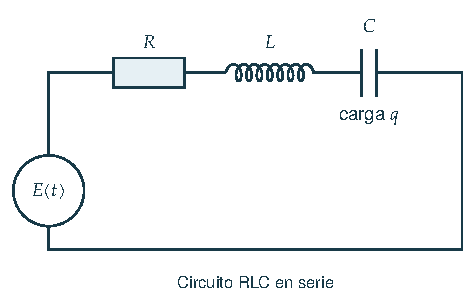
\includegraphics[width=9.02cm]{assets/M2-E0097-setup.pdf}\par
\smallskip{\small Topología del circuito RLC del apartado general.\par}
\end{minipage}
\end{center}
